\section{Evaluation}
\label{sec:evaluation}

\subsection{Research Questions}

We evaluate \sys from three perspectives.
\textbf{RQ1:} How well does \sys infer routes from ASes with no
source-originated path observations available?
\textbf{RQ2:} How well does \sys select egress neighbors and construct
high-quality augmented paths?
\textbf{RQ3:} How effective are the key components of \sys?

\subsection{Experimental Setup}

\subsubsection{Dataset}

We use five monthly BGP snapshots from February 1 to June 1, 2026.
For each date, ten target source ASes yield 685,765--692,950 distinct
source--destination AS queries (Table~\ref{tab:bgp_results}).
The February--April target sets are identical; in May and June,
AS16276 replaces AS42473. The targets have substantial BGP path
coverage, enabling evaluation over many destinations but limiting
generalization to sparsely observed source ASes.

For each target source, its source-originated paths are withheld from
path construction, upstream supervision, and downstream checkpoint
selection. Paths from other origins provide public evidence and
supervision; the resulting augmented paths train the target's route
model. The held-out target paths are used only for the evaluations
below. Table~\ref{tab:data_sources} lists the public data sources.
The inherited graph and AS features do not have complete
origin-level provenance, so source separation is guaranteed for path
labels but not for every graph feature.

\subsubsection{Metrics}
\label{sec:metrics}

For a query $q=(s,d)$, let $\mathcal Y_q$ be its distinct held-out BGP
paths, $\widehat P_q$ the predicted path, and $Q$ the fixed query set
for one date.

\textbf{Inference performance (RQ1).}
\emph{Accuracy (ACC)} is the mean AS-set Jaccard similarity to the
best-matching held-out path:
\begin{equation}
\mathrm{ACC}=\frac{1}{|Q|}\sum_{q\in Q}
       \max_{Y\in\mathcal Y_q}
       \frac{|S(\widehat P_q)\cap S(Y)|}
            {|S(\widehat P_q)\cup S(Y)|}.
\label{eq:jaccard}
\end{equation}
Here $S(P)$ is the set of ASes in $P$, including both endpoints. A
missing, cyclic, or endpoint-invalid prediction scores zero.
\emph{Exact Same Ratio (ESR)} is the fraction of queries with a
best-matching Jaccard score of one.
\emph{Coverage} is the fraction of queries with a valid prediction.
All three metrics use queries, rather than source ASes, as their
weighting unit.

\textbf{Path augmentation quality (RQ2).}
\emph{First-Hop Coverage (FHC)} measures whether selected neighbors
cover the first hops of held-out paths: for each query, we compute
the fraction of paths in $\mathcal Y_q$ whose first hop is selected,
then average equally over queries.
\emph{Neighbor Representation Rate (NRR)} is the fraction of neighbors
that are both selected and observed in held-out paths for which at
least one admitted augmented path uses that first hop. Its numerator
and denominator are pooled over the ten target sources. Neighbors not
observed in the held-out paths are excluded from the denominator.
\emph{Complete-Path Support (CPS)} is the fraction of admitted
augmented paths whose full AS sequence matches a held-out BGP path:
\begin{equation}
\mathrm{CPS}=\frac{|\{P\in\mathcal L^Q:P\in
             \mathcal Y_{(P_0,P_{\rm last})}\}|}
        {|\mathcal L^Q|},
\label{eq:library_support}
\end{equation}
where $\mathcal L^Q$ contains admitted paths whose endpoint pair
appears in the held-out BGP data. Selected-neighbor counts and admitted
path counts describe the scale of the constructed library.

\textbf{Component effectiveness (RQ3).}
\emph{Oracle Accuracy (OA)} is the query-averaged best Jaccard score
among generated candidates before final selection, with zero for a
query without candidates. We also report the selected path's ACC and
ESR for each ablation.

\subsubsection{Baselines}

\emph{KnownPath} infers AS paths from observed BGP paths under routing
constraints~\cite{qiu2005path}. Its index uses the permitted
training-origin BGP paths.
\emph{PathRadar} combines policy-based and path-stitching inference
according to routing observation adequacy~\cite{11044440}. We compare
both baselines on all five dates.
For a given date, every reported method is scored on the same fixed
set of target source--destination AS pairs.

\subsection{Inference Performance Evaluation}
\label{sec:results}

\begin{table}[t]
\centering
\caption{End-to-end BGP path inference across five snapshots.}
\label{tab:bgp_results}
\footnotesize
\renewcommand{\arraystretch}{1.12}
\setlength{\tabcolsep}{2pt}
\begin{tabular*}{\columnwidth}{@{\extracolsep{\fill}}llrrrr@{}}
\toprule
Date & Method & Accuracy & ESR & Queries & Coverage\\
\midrule
\multirow{3}{*}{Feb.} & KnownPath & 71.78\% & 17.55\% & 685,820 & 99.81\%\\
 & PathRadar & 68.93\% & 26.84\% & 685,820 & 99.76\%\\
 & \textbf{\sys} & \textbf{84.52\%} & \textbf{56.64\%} & 685,820 & 99.73\%\\
\midrule
\multirow{3}{*}{Mar.} & KnownPath & 70.52\% & 13.99\% & 685,765 & 99.82\%\\
 & PathRadar & 67.86\% & 25.26\% & 685,765 & 99.80\%\\
 & \textbf{\sys} & \textbf{84.30\%} & \textbf{56.14\%} & 685,765 & 99.73\%\\
\midrule
\multirow{3}{*}{Apr.} & KnownPath & 71.42\% & 17.06\% & 688,302 & 99.81\%\\
 & PathRadar & 69.99\% & 28.05\% & 688,302 & 99.76\%\\
 & \textbf{\sys} & \textbf{83.17\%} & \textbf{54.18\%} & 688,302 & 99.63\%\\
\midrule
\multirow{3}{*}{May} & KnownPath & 70.58\% & 14.61\% & 692,950 & 99.77\%\\
 & PathRadar & 71.00\% & 28.96\% & 692,950 & 99.75\%\\
 & \textbf{\sys} & \textbf{83.14\%} & \textbf{52.71\%} & 692,950 & 99.64\%\\
\midrule
\multirow{3}{*}{Jun.} & KnownPath & 71.06\% & 15.65\% & 692,497 & 99.73\%\\
 & PathRadar & 70.08\% & 26.82\% & 692,497 & 99.76\%\\
 & \textbf{\sys} & \textbf{83.12\%} & \textbf{52.41\%} & 692,497 & 99.58\%\\
\bottomrule
\end{tabular*}
\end{table}


\sys attains 83.12--84.52\% ACC and 52.41--56.64\% ESR across the
five snapshots, with 99.58--99.73\% Coverage
(Table~\ref{tab:bgp_results}). KnownPath attains 70.52--71.78\% ACC,
giving \sys an 11.75--13.79 percentage-point gain on the same query
sets. PathRadar attains 67.86--71.00\% ACC and 25.26--28.96\% ESR.
\sys improves ACC over PathRadar by 12.14--16.44 points across the
five dates.

\begin{figure*}[t]
\centering
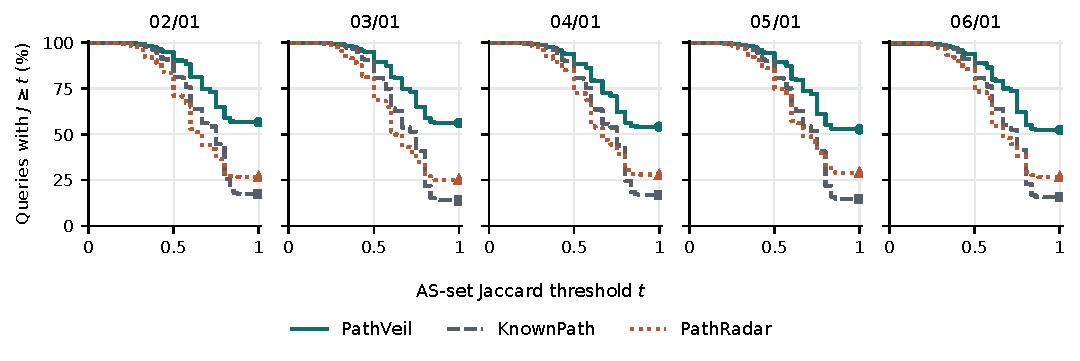
\includegraphics[width=\textwidth]{figures/fig_query_jaccard_distribution.pdf}
\caption{Per-query AS-set Jaccard distributions across five BGP
snapshots. Each panel shows the fraction of queries with score
$J\geq t$. Missing predictions score zero; the value at $t=1$ is
ESR, and the area under a curve is ACC.}
\label{fig:query_distribution}
\end{figure*}

Figure~\ref{fig:query_distribution} shows the distribution behind
these averages. \sys retains more queries at high Jaccard thresholds
on all five dates. In February, 56.64\% of its queries reach $J=1$,
compared with 17.55\% for KnownPath and 26.84\% for PathRadar.
KnownPath's higher ACC than ESR indicates that many of its routes
share some ASes with a held-out path without matching its full AS set.

\subsection{Path Augmentation Quality Evaluation}

\begin{table}[t]
\centering
\caption{Neighbor selection and augmented-path assessment.}
\label{tab:stage_results}
\footnotesize
\renewcommand{\arraystretch}{1.12}
\begin{tabular*}{\columnwidth}{@{\extracolsep{\fill}}lrrrrr@{}}
\toprule
Date & Sel. nbrs. & Aug. paths & FHC & NRR & CPS\\
\midrule
Feb. & 17.2 & 38,175 & 85.02\% & 93.41\% & 95.62\%\\
Mar. & 17.4 & 33,299 & 84.54\% & 95.78\% & 89.25\%\\
Apr. & 17.4 & 33,264 & 83.33\% & 94.61\% & 91.51\%\\
May & 17.5 & 30,128 & 81.60\% & 92.35\% & 93.41\%\\
Jun. & 17.4 & 30,551 & 81.61\% & 92.94\% & 94.04\%\\
\bottomrule
\end{tabular*}
\end{table}


Table~\ref{tab:stage_results} evaluates RQ2. Across the five dates,
the selected neighbors cover 81.60--85.02\% of held-out first-hop
choices (FHC). Among selected neighbors observed in the held-out
paths, 92.35--95.78\% receive at least one admitted augmented path
(NRR). The library contains 30,128--38,175 paths per date, with an
average of 17.2--17.5 selected neighbors per target source.

Complete-path support (CPS) is 89.25--95.62\% among augmented paths
whose source--destination pair appears in the held-out data. This
measure checks the entire AS sequence, whereas FHC and NRR assess
only first-hop selection and representation. The held-out BGP corpus
is finite: a nonmatch does not prove that a constructed path is
impossible, and a match does not establish packet forwarding. CPS
also includes paths found intact in public observations, so it does
not isolate the quality of newly stitched joins.

\begin{figure}[t]
\centering
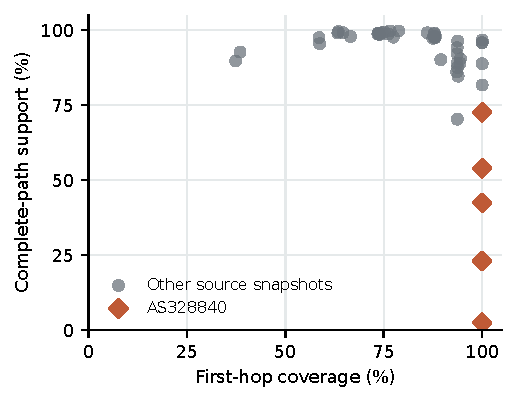
\includegraphics[width=\columnwidth]{figures/fig_eval_stage.pdf}
\caption{First-hop coverage does not guarantee complete-path support.
Each point is one target AS on one date; AS328840 is highlighted.}
\label{fig:eval_stage}
\end{figure}

Figure~\ref{fig:eval_stage} exposes an important failure case:
AS328840 has nearly complete FHC on every date, but its CPS ranges
from 2.40\% in April to 72.53\% in February. Selecting a relevant
egress neighbor therefore does not by itself ensure that the
constructed route beyond that neighbor agrees with observations.

\subsection{Component Ablation}

To answer RQ3, we vary recursive exploration and candidate generation
separately. The recursion ablation compares conditional expansion with
no expansion and expansion at every selected first-hop neighbor.
The generator ablation replaces prefix-tree-constrained generation
with the prior high-frequency-node path generator (PG), keeping the
admitted training library and recursion policy fixed. All variants
are scored on the same query pairs within each date.

\begin{table}[t]
\centering
\caption{Recursive exploration ablation (query-weighted \%).}
\label{tab:ablation_recursion}
\footnotesize
\setlength{\tabcolsep}{3pt}
\renewcommand{\arraystretch}{1.08}
\begin{tabular*}{\columnwidth}{@{\extracolsep{\fill}}llrrr@{}}
\toprule
Date & Expansion & Oracle ACC & Accuracy & ESR\\
\midrule
\multirow{3}{*}{Feb.} & Conditional & 98.70 & \textbf{84.52} & \textbf{56.64}\\
 & None & 93.12 & 80.39 & 48.44\\
 & All & 98.72 & 84.02 & 54.74\\
\midrule
\multirow{3}{*}{Mar.} & Conditional & 98.12 & \textbf{84.30} & \textbf{56.14}\\
 & None & 92.63 & 81.84 & 51.69\\
 & All & 98.15 & 83.89 & 54.95\\
\midrule
\multirow{3}{*}{Apr.} & Conditional & 97.95 & 83.17 & 54.18\\
 & None & 92.40 & 81.63 & 51.53\\
 & All & 97.97 & \textbf{83.46} & \textbf{54.63}\\
\midrule
\multirow{3}{*}{May} & Conditional & 97.79 & 83.14 & 52.71\\
 & None & 93.81 & 82.20 & 50.83\\
 & All & 97.80 & \textbf{83.30} & \textbf{53.51}\\
\midrule
\multirow{3}{*}{Jun.} & Conditional & 97.73 & 83.12 & 52.41\\
 & None & 92.00 & 79.16 & 44.15\\
 & All & 97.74 & \textbf{83.93} & \textbf{54.51}\\
\bottomrule
\end{tabular*}
\end{table}


\begin{figure*}[t]
\centering
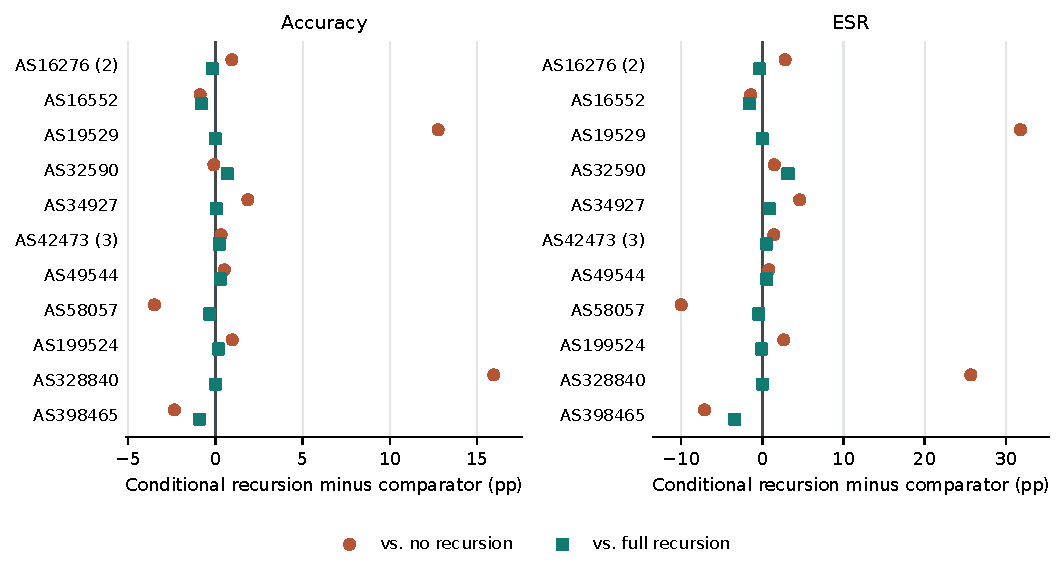
\includegraphics[width=\textwidth]{figures/fig_ablation_recursion.pdf}
\caption{No recursion vs. conditional recursion (circles) and full
recursion vs. conditional recursion (squares), in ACC (left) and ESR
(right). Each point plots conditional recursion minus the comparator,
so positive values favor conditional recursion. Scores pool each
source's queries across available dates; AS42473 occurs in
February--April and AS16276 in May--June.}
\label{fig:ablation_recursion}
\end{figure*}

Removing recursion lowers ACC on every date by 0.94--4.13 percentage
points (Table~\ref{tab:ablation_recursion}). Full recursion attains
nearly the same OA as conditional recursion, and their final ACC
differs by at most 0.81 points. Conditional recursion performs
better in February and March; full recursion performs better from
April through June. Thus, exploration is useful, while the
conditional policy has no consistent accuracy advantage over
expanding every selected neighbor. Figure~\ref{fig:ablation_recursion}
shows that its effect also varies across source ASes.

\begin{table}[t]
\centering
\caption{Candidate-generation ablation (query-weighted \%).}
\label{tab:ablation_generator}
\footnotesize
\setlength{\tabcolsep}{3pt}
\renewcommand{\arraystretch}{1.08}
\begin{tabular*}{\columnwidth}{@{\extracolsep{\fill}}llrrr@{}}
\toprule
Date & Generator & Oracle ACC & Accuracy & ESR\\
\midrule
\multirow{2}{*}{Feb.} & Prefix tree & \textbf{98.70} & \textbf{84.52} & \textbf{56.64}\\
 & PG & 91.43 & 77.02 & 35.54\\
\midrule
\multirow{2}{*}{Mar.} & Prefix tree & \textbf{98.12} & \textbf{84.30} & \textbf{56.14}\\
 & PG & 91.35 & 77.85 & 39.88\\
\midrule
\multirow{2}{*}{Apr.} & Prefix tree & \textbf{97.95} & \textbf{83.17} & \textbf{54.18}\\
 & PG & 90.12 & 75.21 & 33.82\\
\midrule
\multirow{2}{*}{May} & Prefix tree & \textbf{97.79} & \textbf{83.14} & \textbf{52.71}\\
 & PG & 91.20 & 76.11 & 34.89\\
\midrule
\multirow{2}{*}{Jun.} & Prefix tree & \textbf{97.73} & \textbf{83.12} & \textbf{52.41}\\
 & PG & 89.64 & 76.15 & 35.26\\
\bottomrule
\end{tabular*}
\end{table}


\begin{figure*}[t]
\centering
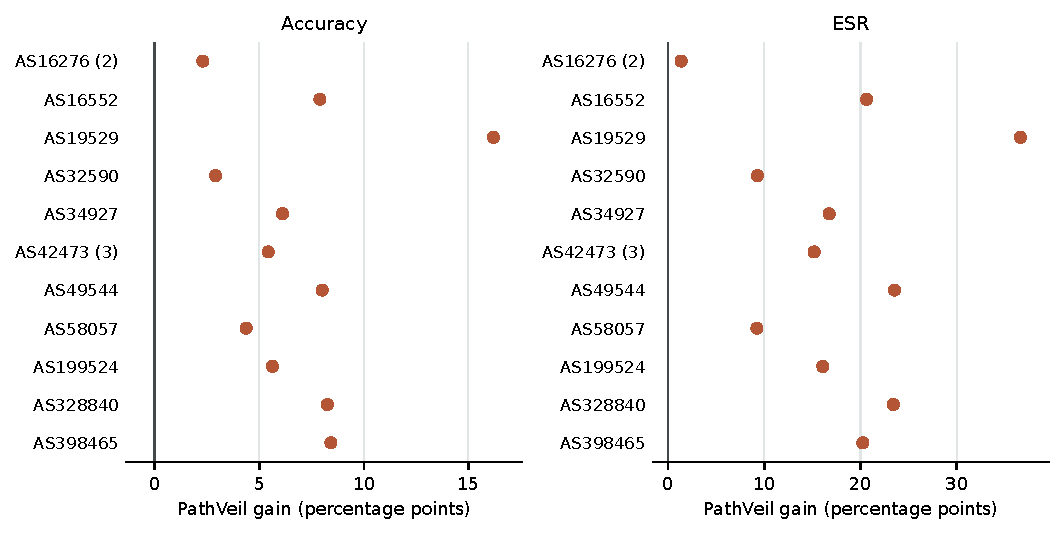
\includegraphics[width=\textwidth]{figures/fig_ablation_generator.pdf}
\caption{Per-source ACC gain from prefix-tree-constrained generation
over PG, with the same recursion policy and admitted path library.
Each point averages the source's dated queries.}
\label{fig:ablation_generator}
\end{figure*}

Replacing the prefix-tree generator with PG lowers OA by
6.59--8.09 points across the five dates
(Table~\ref{tab:ablation_generator}). ACC falls by 6.45--7.96
points and ESR by 16.26--21.10 points. The candidate-space loss
therefore carries through to the selected prediction.
Figure~\ref{fig:ablation_generator} shows that the size of this
gain differs by source AS.
